\documentclass{article}

  % packages
    % basic stuff for rendering math
    \usepackage[letterpaper, top=1in, bottom=1in, left=1in, right=1in]{geometry}
    \usepackage[utf8]{inputenc}
    \usepackage[english]{babel}
    \usepackage{amsmath} 
    \usepackage{amssymb}
    \usepackage{bookmark}

    % extra math symbols and utilities
    \usepackage{mathtools}        % for extra stuff like \coloneqq
    \usepackage{mathrsfs}         % for extra stuff like \mathsrc{}
    \usepackage{centernot}        % for the centernot arrow 
    \usepackage{bm}               % for better boldsymbol/mathbf 
    \usepackage{enumitem}         % better control over enumerate, itemize
    \usepackage{hyperref}         % for hypertext linking
    \usepackage{xr-hyper}
    \usepackage{fancyvrb}          % for better verbatim environments
    \usepackage{newverbs}         % for texttt{}
    \usepackage{xcolor}           % for colored text 
    \usepackage{listings}         % to include code
    \usepackage{lstautogobble}    % helper package for code
    \usepackage{parcolumns}       % for side by side columns for two column code
    \usepackage{algorithm}
    \usepackage{algpseudocode}
    \usepackage{bbm}
    \algblock{Class}{EndClass}

    % page layout
    \usepackage{fancyhdr}         % for headers and footers 
    \usepackage{uniquecounter}
    \usepackage{lastpage}         % to include last page number in footer 
    \usepackage{parskip}          % for no indentation and space between paragraphs   
    \usepackage[T1]{fontenc}      % to include \textbackslash
    \usepackage{footnote}
    \usepackage{etoolbox}

    % for custom environments
    \usepackage{tcolorbox}        % for better colored boxes in custom environments
    \tcbuselibrary{breakable}     % to allow tcolorboxes to break across pages

    % figures
    \usepackage{pgfplots}
    \pgfplotsset{compat=1.18}
    \usepackage{float}            % for [H] figure placement
    \usepackage{tikz}
    \usepackage{tikz-cd}
    \usepackage{circuitikz}
    \usetikzlibrary{arrows, arrows.meta}
    \usetikzlibrary{positioning}
    \usetikzlibrary{calc}
    \usepackage{graphicx}
    \usepackage{caption} 
    \usepackage{subcaption}
    \captionsetup{font=small} 

    % for tabular stuff 
    \usepackage{dcolumn}

    \usepackage[nottoc]{tocbibind}
    \pdfsuppresswarningpagegroup=1
    \hfuzz=5.002pt                % ignore overfull hbox badness warnings below this limit

  % New and replaced operators
    \DeclareMathOperator{\Tr}{Tr}
    \DeclareMathOperator{\Sym}{Sym}
    \DeclareMathOperator{\Span}{span}
    \DeclareMathOperator{\elbo}{ELBO}
    \DeclareMathOperator{\std}{std}
    \DeclareMathOperator{\Cov}{Cov}
    \DeclareMathOperator{\Var}{Var}
    \DeclareMathOperator{\Corr}{Corr}
    \DeclareMathOperator{\pos}{pos}
    \DeclareMathOperator*{\argmin}{\arg\!\min}
    \DeclareMathOperator*{\argmax}{\arg\!\max}
    \newcommand{\qed}{\hfill$\blacksquare$}     % I like QED squares to be black

  % Custom Environments
    \newtcolorbox[auto counter, number within=section]{question}[1][]
    {
      colframe = orange!25,
      colback  = orange!10,
      coltitle = orange!20!black,  
      breakable, 
      title = \textbf{Question \thetcbcounter ~(#1)}
    }

    \newtcolorbox[auto counter, number within=section]{exercise}[1][]
    {
      colframe = teal!25,
      colback  = teal!10,
      coltitle = teal!20!black,  
      breakable, 
      title = \textbf{Exercise \thetcbcounter ~(#1)}
    }
    \newtcolorbox[auto counter, number within=section]{solution}[1][]
    {
      colframe = violet!25,
      colback  = violet!10,
      coltitle = violet!20!black,  
      breakable, 
      title = \textbf{Solution \thetcbcounter}
    }
    \newtcolorbox[auto counter, number within=section]{lemma}[1][]
    {
      colframe = red!25,
      colback  = red!10,
      coltitle = red!20!black,  
      breakable, 
      title = \textbf{Lemma \thetcbcounter ~(#1)}
    }
    \newtcolorbox[auto counter, number within=section]{theorem}[1][]
    {
      colframe = red!25,
      colback  = red!10,
      coltitle = red!20!black,  
      breakable, 
      title = \textbf{Theorem \thetcbcounter ~(#1)}
    } 
    \newtcolorbox[auto counter, number within=section]{corollary}[1][]
    {
      colframe = red!25,
      colback  = red!10,
      coltitle = red!20!black,  
      breakable, 
      title = \textbf{Corollary \thetcbcounter ~(#1)}
    } 
    \newtcolorbox[auto counter, number within=section]{proof}[1][]
    {
      colframe = orange!25,
      colback  = orange!10,
      coltitle = orange!20!black,  
      breakable, 
      title = \textbf{Proof. }
    } 
    \newtcolorbox[auto counter, number within=section]{definition}[1][]
    {
      colframe = yellow!25,
      colback  = yellow!10,
      coltitle = yellow!20!black,  
      breakable, 
      title = \textbf{Definition \thetcbcounter ~(#1)}
    } 
    \newtcolorbox[auto counter, number within=section]{example}[1][]
    {
      colframe = blue!25,
      colback  = blue!10,
      coltitle = blue!20!black,  
      breakable, 
      title = \textbf{Example \thetcbcounter ~(#1)}
    } 
    \newtcolorbox[auto counter, number within=section]{code}[1][]
    {
      colframe = green!25,
      colback  = green!10,
      coltitle = green!20!black,  
      breakable, 
      title = \textbf{Code \thetcbcounter ~(#1)}
    } 
    \newtcolorbox[auto counter, number within=section]{algo}[1][]
    {
      colframe = green!25,
      colback  = green!10,
      coltitle = green!20!black,  
      breakable, 
      title = \textbf{Algorithm \thetcbcounter ~(#1)}
    } 
    \definecolor{cverbbg}{gray}{0.93}
    \newenvironment{cverbatim}
      {\SaveVerbatim{cverb}}
      {\endSaveVerbatim
        \flushleft\fboxrule=0pt\fboxsep=.5em
        \colorbox{cverbbg}{%
          \makebox[\dimexpr\linewidth-2\fboxsep][l]{\BUseVerbatim{cverb}}%
        }
        \endflushleft
    }

    \definecolor{dkgreen}{rgb}{0,0.6,0}
    \definecolor{gray}{rgb}{0.5,0.5,0.5}
    \definecolor{mauve}{rgb}{0.58,0,0.82}
    \definecolor{lightgray}{gray}{0.93}
    \renewcommand{\algorithmiccomment}[1]{\hfill$\triangleright$\textcolor{blue}{#1}}

    % default options for listings (for code)
    \lstset{
      autogobble,
      frame=ltbr,
      language=Python,                           % the language of the code
      aboveskip=3mm,
      belowskip=3mm,
      showstringspaces=false,
      columns=fullflexible,
      keepspaces=true,
      basicstyle={\small\ttfamily},
      numbers=left,
      firstnumber=1,                        % start line number at 1
      numberstyle=\tiny\color{gray},
      keywordstyle=\color{blue},
      commentstyle=\color{dkgreen},
      stringstyle=\color{mauve},
      backgroundcolor=\color{lightgray}, 
      breaklines=true,                      % break lines
      breakatwhitespace=true,
      tabsize=3, 
      xleftmargin=2em, 
      framexleftmargin=1.5em, 
      stepnumber=1
    }

  % Page style
    \pagestyle{fancy}
    \fancyhead[L]{Normalizing Flows}
    \fancyhead[C]{Muchang Bahng}
    \fancyhead[R]{Spring 2023} 
    \fancyfoot[C]{\thepage / \pageref{LastPage}}
    \renewcommand{\footrulewidth}{0.4pt}          % the footer line should be 0.4pt wide
    \renewcommand{\thispagestyle}[1]{}  % needed to include headers in title page
%    \renewcommand{\thefootnote}{\arabic{footnote}}

  % external documents 
    \externaldocument[algo-]{../../Computer_Science/DSA/paper}[../../Computer_Science/DSA/paper.pdf]

\begin{document}

\tikzset{every picture/.style={line width=0.75pt}} 

\title{Normalizing Flows}
\author{Muchang Bahng}
\date{Spring 2023}

\maketitle
\tableofcontents
\pagebreak 


This covers computability theory, complexity theory, and automata theory. 
Alphabet. Boolean logic



\section{Normalizing Flows} 

  We have seen many examples of generative models that attempt to produce a probability distribution $p$ that approximates the true pdf $p^\ast$ of the data samples. Some are given by an explicit model (e.g. GMMs, RBMs, VAEs) which approximate with parameterized form $p^\ast \sim p_\theta$, while in others (GANs) the model is implicit since we model the random variable as a transformation $X = G_{g_\theta} (Z)$ through a neural network with $Z \sim \mathcal{N}(0, I)$. If we focus on VAEs---specifically variational inference---for a second, recall that the performance of the model really just depends on the fact that we can approximate the intractable posterior $p(z \mid x)$ with some parameterized family $q_\phi (z)$\footnote{This can be written $q_\phi (z) = q_\phi (z \mid x)$, but since the encoder network produces the $\phi = E_\alpha (x)$, the $q_\phi(z)$ really represents a conditional distribution given $x$.} 

  \begin{equation}
    \elbo(x^{(i)}, \phi, \theta) = \underbrace{\mathbb{E}_{q_\phi (z \mid x^{(i)})} [\log p_{\theta} (x^{(i)} \mid z)]}_{\substack{\text{likelihood term} \\ \text{(reconstruction part)}}}- \underbrace{KL(q_{\phi} (z \mid x^{(i)}) \mid\mid p(z))}_{\substack{\text{closeness of encoding to } p(z) \\ \text{(typically Gaussian)}}}
  \end{equation}
  This may not be advantageous and flexible enough to capture the true posterior if $q_\phi(z)$ is far away from $p(z \mid x)$

  To address this problem, in 2015, Google Deepmind through \cite{flow} introduced the idea of \textit{flow-based} models \footnote{This has nothing to do with flow graphs and the max-flow-min-cut theorem in graph theory.} which---like GANs---want to map simple distributions (e.g. a Gaussian) to complex densities representing the data. This would normally result in an implicitly defined pdf, but by making the transformation to be \textit{invertible}, we can use the change of basis formula to get a closed-form of the pdf, making flow models an \textit{explicit} model of the pdf. Recall the lemma below from multivariate calculus. 
  
  \begin{lemma}[Jacobi] 
    Let $X, Z$ be absolutely continuous random variables in $\mathbb{R}^n$. 
    Given that $f: \mathbb{R}^n \rightarrow \mathbb{R}^n$ is invertible and differentiable everywhere, with $X = f(Z), Z = f^{-1} (X)$, we claim 
    \begin{equation}
      p_X (x) = p_Z (z) \cdot \bigg| \det \frac{\partial f^{-1}}{\partial x} \bigg| = p_Z (z) \cdot \bigg| \det \frac{\partial f}{\partial z}  \bigg|^{-1}
    \end{equation} 
    where $\det$ is the determinant of the total derivative (Jacobian). 
  \end{lemma}
  \begin{proof}
    For $n = 1$, we have 
    \begin{align}
      p_X (x) & = \frac{d}{dx} F_X (x) \\
              & = \frac{d}{dx} F_Z (f^{-1}(x)) \\
              & = p_z (f^{-1} (x)) \cdot \frac{d}{dx} f^{-1} (x)  \\
              & = p_z 
    \end{align}
  \end{proof} 

  Therefore, if we parameterize $f$ with some $\theta$, then the marginal likelihood of $x$ given $\theta$ can be written as 
  \begin{equation}
    p_X (x;\; \theta) = p_Z (f^{-1}_\theta (x)) \cdot \bigg| \det \frac{\partial f_\theta^{-1}}{\partial x} \bigg|
  \end{equation} 
  Therefore, if $X$ is a complex distribution and $Z$ is a simple one (e.g. uniform), we might have hope to efficiently compute $p_X (x)$ for any $x \in \mathbb{R}^n$ if 
  \begin{enumerate}
    \item we can efficiently compute $f^{-1}_\theta (x)$, which allows us to compute $p_Z (f^{-1} (x))$ efficiently since $Z$ is simple. 
    \item we can efficiently compute the determinant of the Jacobian $|\det (\partial f_\theta^{-1}/\partial x)|$.\footnote{Note that computing determinants are approximately $O(n^{2.4})$, which may not be practical. } 
  \end{enumerate}  

\subsection{Finite Normalizing Flows}

  It looks like we have split this enormously hard problem of modeling $X$ with two slightly less difficult problems. However, with some tricks, we may be able to get a simple enough parameterization of $f$ to be able to compute its inverse plus the determinant of the Jacobian. Note that the construction of a neural network was to take a simple function (one layer) and construct a complex family of functions composed of multiple layers. This is what we can do as well. 

  \begin{corollary}[Finite Normalizing Flow]
    Given a sequence of transformations 
    \begin{equation}
      Z = Z_0 \xrightarrow{f_1} Z_1 \xrightarrow{f_2} \ldots \xrightarrow{f_{K-1}} Z_{K-1} \xrightarrow{f_K} Z_K = X
    \end{equation} 
    where each $f_k$ is invertible and differentiable everywhere, let us denote $f = f_K \circ \ldots \circ f_1: Z \rightarrow X$, which is invertible. Then
    \begin{equation}
      p_X (x) = p_Z (f^{-1} (x)) \cdot \prod_{k=1}^K \bigg| \det \frac{\partial f_k}{ \partial z_{k-1}} \bigg|^{-1}
    \end{equation}
    This sequence of random variables $Z_k$ is called a \textbf{flow}, and the sequence of the corresponding pdfs $p_{Z_k}$ is called the \textbf{normalizing flow}. As for how we parameterize this, our notation will assume that $\theta = (\theta_1, \ldots, \theta_M)$ and each $\theta_m$ parameterizes $f_m$.
  \end{corollary} 
  \begin{proof}
    This can automatically be proved by induction. For an example, consider the sequence of invertible functions $Z \xrightarrow{f} Y \xrightarrow{g} \rightarrow X$, where $Z$ is a simple distribution that gets transformed to a slightly more complicated distribution $Y$ that then gets transformed to a complex distribution $X$. We can apply the Jacobi theorem above to see $p_Y (y) = p_Z (f^{-1} (y)) \cdot | (Df^{-1})(x)|$, and so we have 
    \begin{align}
      p_X (x) & = p_Y (g^{-1} (x)) \cdot | (D g^{-1}) (x) | \\
              & = p_Z (f^{-1} (g^{-1} (x))) \cdot | (Df^{-1}) (y)| \cdot | (D g^{-1}) (x) | \\ 
              & = p_Z ((g \circ f)^{-1} (x))) \cdot | (Df^{-1}) (y)| \cdot | (D g^{-1}) (x) | 
    \end{align}
  \end{proof}

  Therefore, by taking a sequence these functions $f_m$, which may each have a simple parameterization, we may construct a very complex composition $f_\theta$ that may result in a very expressive $Z$. Again, this is very similar to how a composition of linear mappings plus an activation gives us a very expressive neural network, and unsurprisingly, there is an analogue of the universal approximation theorem for transformations of this form. 

  \begin{theorem}[Probability Integral Transform] 
    Any $n$-dimensional random variable in $\mathbb{R}^n$ that is absolutely continuous w.r.t. the Lebesgue measure can be constructed from the uniform distribution $U$ on $[0, 1]^n$. Since we can map to and back from invertibility, any two such random variables $X$ and $Y$ can be mapped from each other, 
    \begin{equation}
      X \mapsto U \mapsto Y 
    \end{equation}
  \end{theorem} 

  Now given this, our job is to maximize the log-likelihood. Since $x = z_K$ and $z = z_0$, we substitute this in 
  \begin{equation}
    \ln p_{Z_K} (x) = \ln p_{Z_0} (f^{-1}(x)) - \sum_{k=1}^K \ln \bigg| \det \frac{\partial f_k}{\partial z_{k-1}} \bigg| 
  \end{equation} 
  and over the dataset we want to find 
  \begin{equation}
    f^\ast = \argmax_{f} \sum_{i=1}^N \ln p_{Z_0} (f^{-1}(x^{(i)})) - \sum_{k=1}^K \ln \bigg| \det \frac{\partial f_k}{\partial z_{k-1}} \bigg| 
  \end{equation}
  where we are really optimizing over $f_1, \ldots, f_K$, i.e. their parameters $\theta_1, \ldots, \theta_K$. Great, now let's define the parametric form of $f$. There are two different types of invertible transformations that we can calculate in linear time. 

  \begin{definition}[Planar Contractions]
    Let us have $\theta = \{w \in \mathbb{R}^D, u \in \mathbb{R}^D, b \in \mathbb{R}\}$ and define the family of \textbf{planar contractions}
    \begin{equation}
      \{f(z) = z + u \cdot h( w^T z + b)\}_\theta
    \end{equation}
    for some smooth nonlinearity $h$.\footnote{As the paper states, this flow can be visualized as modifying the initial density by applying a series of contractions and expansions in the direction perpendicular to the hyperplane $w^T z + b$.} This is not always invertible, but the paper uses $h(x) = \tanh(x)$ with the fact that $w^T u \geq -1$ is sufficient for $f$ to be invertible. 
  \end{definition} 
  
  This already looks like a single layer, so you might wonder why one can't just directly make an invertible neural net? There is already literature on this, but the typical computational complexity of computing the determinant (plus the gradient of the determinant) is of scale $O(LD^3)$, where $L$ is the number of hidden layers and $D$ is the dimension of each hidden layer. It turns out that this decomposition gives us a very cute formula for computing determinants. 

  \begin{lemma}
    The determinant of a planar contraction is 
    \begin{equation}
      \bigg| \det \frac{\partial f}{\partial z} \bigg| = \big| \det (I + u \psi (z)^T ) \big| = \big| 1 + u^T \psi(z) \big| 
    \end{equation} 
    where $\psi(z) = h^\prime (w^T z + b) \cdot w$. This can be computed in $O(D)$ time. 
  \end{lemma}
  \begin{proof}
    Use block matrix multiplication and the \href{https://en.wikipedia.org/wiki/Matrix_determinant_lemma}{matrix determinant lemma}.
  \end{proof}

  The other type mentioned is a radial contraction. 

  \begin{definition}[Radial Contraction]
    Let us have $\theta = \{ c \in \mathbb{R}^D, \alpha \in \mathbb{R}^+, \beta \in \mathbb{R} \}$ and define the family of \textbf{radial contractions} 
    \begin{equation}
      \{ f(z) = z + \beta h(\alpha, r) (z - c) \}_\theta
    \end{equation}
    where $r = |z - c|$ and $h(\alpha, r) = \frac{1}{\alpha + r}$.\footnote{It applies radial contractions and expansions around the reference point $c$ and are referred to as radial flows. }
  \end{definition}

  \begin{lemma} 
    The determinant of a radial contraction is 
    \begin{equation}
      \bigg| \det \frac{\partial f}{\partial z} \bigg| = \big[ 1 + \beta h(\alpha, r)\big]^{d-1} \big[ 1 + \beta h(\alpha, r) + \beta h^\prime (\alpha, r) r \big]
    \end{equation}
  \end{lemma}

  \begin{figure}[H]
    \centering 
    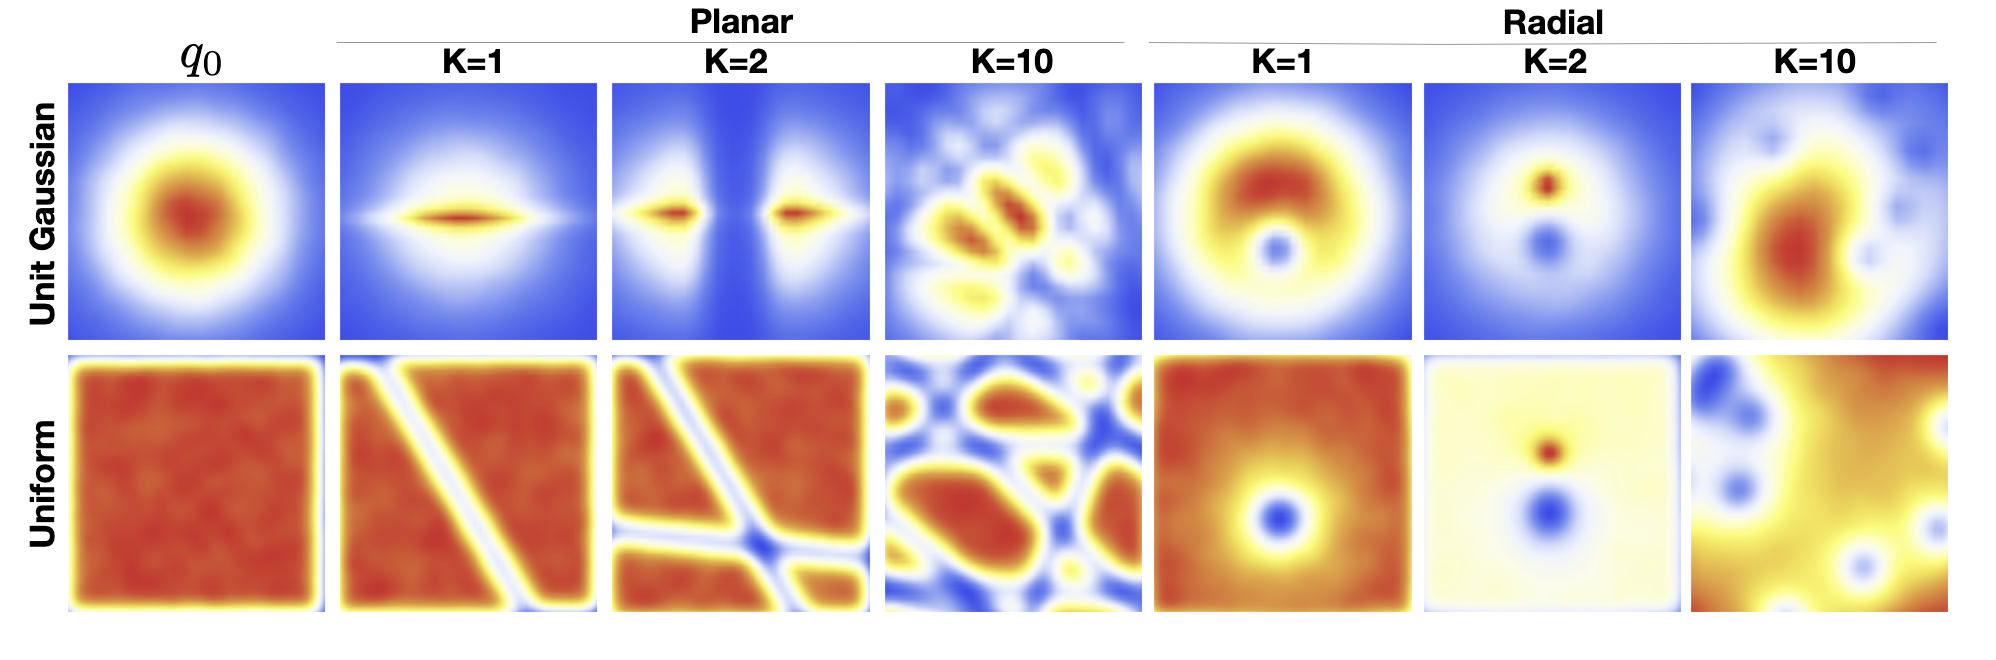
\includegraphics[scale=0.4]{img/contractions.png}
    \caption{The effects of normalizing flow on two distributions. For example, for $k=2$ we can transform a spherical Gaussian into a bimodal distribution by applying 2 successive transformations. } 
    \label{fig:contractions}
  \end{figure} 

  With this form, we can now substitute this into the variational lower bound. Note that we have not just simplified it with the following theorem, but we have also set it up as an expectation over the initial density $p(z)$, analogous to the reparamaterization trick that we have used for VAEs. 

  \begin{theorem}
    The variational lower bound can be written in the simplified form where the 
    \begin{equation}
      \elbo(x) = \mathbb{E}_{q_0 (z_0)} [ \log q_0 (z_0)] - \mathbb{E}_{q_0 (z_0)} [ \log p(x, z_K)] - \mathbb{E}_{q_0 (z_0)} \bigg[ \sum_{k=1}^K \log \big| 1 + u_k^T \psi_k (z_{k-1}) \big| \bigg]
    \end{equation}
    for flow models. 
  \end{theorem}
  \begin{proof}
    By definition $q_\phi(z \mid x) \coloneqq q_K (z_k)$, and substituting this in along with our simplified formula for the log likelihood gives us 
    \begin{align}
      \elbo(x) & \coloneqq \mathbb{E}_{q_\phi (z \mid x)} \big[ \log q_\phi (z \mid x) - \log p(x, z) \big] \\
               & = \mathbb{E}_{q_K (z_K)} \big[ \log q_K (z_K) \big] - \mathbb{E}_{q_K (z_K)} \big[ \log p(x, z_K) \big]  \\ 
               & = \mathbb{E}_{q_K (z_K)}  \bigg[ \log q_0 (z_0) - \sum_{k=1}^K \log \big| 1 + u_k^T \psi_k (z_{k-1}) \big| \bigg] - \mathbb{E}_{q_K (z_K)} \big[ \log p(x, z_K) \big] 
    \end{align}
    But since $z_K = f(z_0)$, using LOTUS we can get 
    \begin{equation}
      \elbo(x) = \mathbb{E}_{q_0 (z_0)} [\log q_0 (z_0)] - \mathbb{E}_{q_0 (z_0)}  \bigg[ \sum_{k=1}^K \log \big| 1 + u_k^T \psi_k (z_{k-1}) \big| \bigg] - \mathbb{E}_{q_0 (z_0)} \big[ \log p(x, z_K) \big] 
    \end{equation}
  \end{proof} 

  At this point we can take the gradients, freely swap them with the expectations, and compute them. 

\subsection{Coupling-Layer Flows} 

    This general method allowing linear-time computation of Jacobian determinants is an example of a \textbf{general normalizing flow}. Before, we have just constructed some family of invertible functions $\{f\}$ to transform the data, such that it was simple enough to calculate the Jacobian determinants in linear time. But note that in general, computing determinants requires you to have an triangular matrix (multiply all the diagonals). Therefore, if we can create a neural network $f$ such that its Jacobian is triangular, we will be done. In order to have such an architecture to support this, we should introduce a special type of layer.  

    \begin{definition}[Affine Coupling Layer]
      Let us have an input $z \in \mathbb{R}^D$ such that it can be partitioned into its first $d$ elements and the rest. 
      \begin{equation}
        z = [z_{1:d}, z_{d+1:D}]
      \end{equation}
      Now let's have 2 neural networks (not necessarily invertible) $F: \mathbb{R}^d \rightarrow \mathbb{R}^{D-d}$ and $H: \mathbb{R}^d \rightarrow \mathbb{R}^{D-d}$ defined 
      \begin{align}
        F(z^\prime) = \beta, \qquad G(z^\prime) = \gamma
      \end{align}
      Then the \textbf{coupling layer} $g: \mathbb{R}^D \rightarrow \mathbb{R}^D$ with parameters $\theta = (\theta_F, \theta_H)$ is defined as the transformation $x = g(z)$, where
      \begin{align}
        x_{1:d} & = z_{1:d} \\ 
        x_{d+1:D} & = z_{d+1:D} \odot \beta + \gamma = z_{d+1:D} \odot F(x_{1:d}) + H(x_{d+1:D})
      \end{align}
    \end{definition}

    So this ``layer'' really composes of two neural networks, and it has both properties that we want. It is invertible, with inverse $z = g^{-1} (x)$ defined 
    \begin{equation}
      z^\prime = x^\prime, \qquad \bar{z} = \frac{\bar{z} - \gamma}{\beta} = \frac{\bar{z} - H(z^\prime)}{F(z^\prime)} 
    \end{equation} 

    \begin{figure}[H]
      \centering
      \begin{subfigure}[b]{0.48\textwidth}
      \centering
        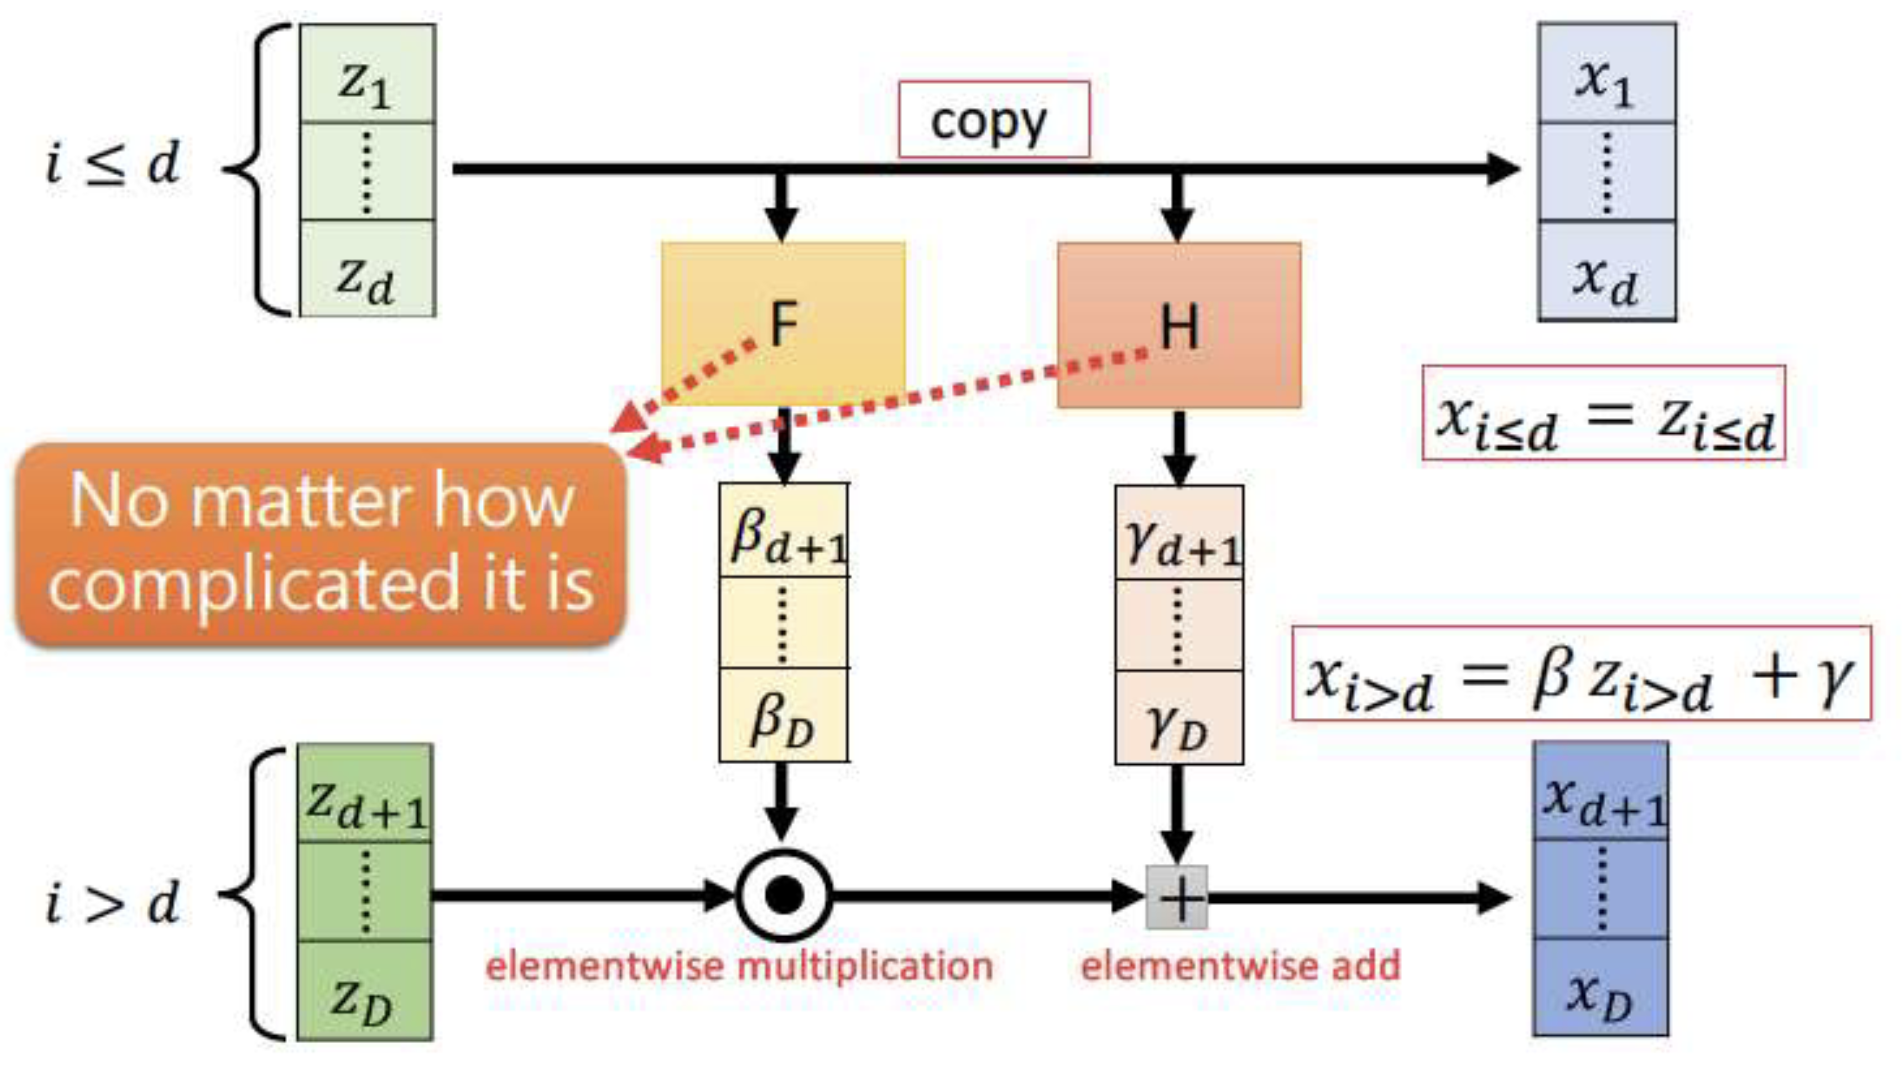
\includegraphics[width=\textwidth]{img/couple_forward.png}
        \caption{Forward pass of the coupling layer.}
        \label{fig:for}
      \end{subfigure}
      \hfill 
      \begin{subfigure}[b]{0.48\textwidth}
      \centering
        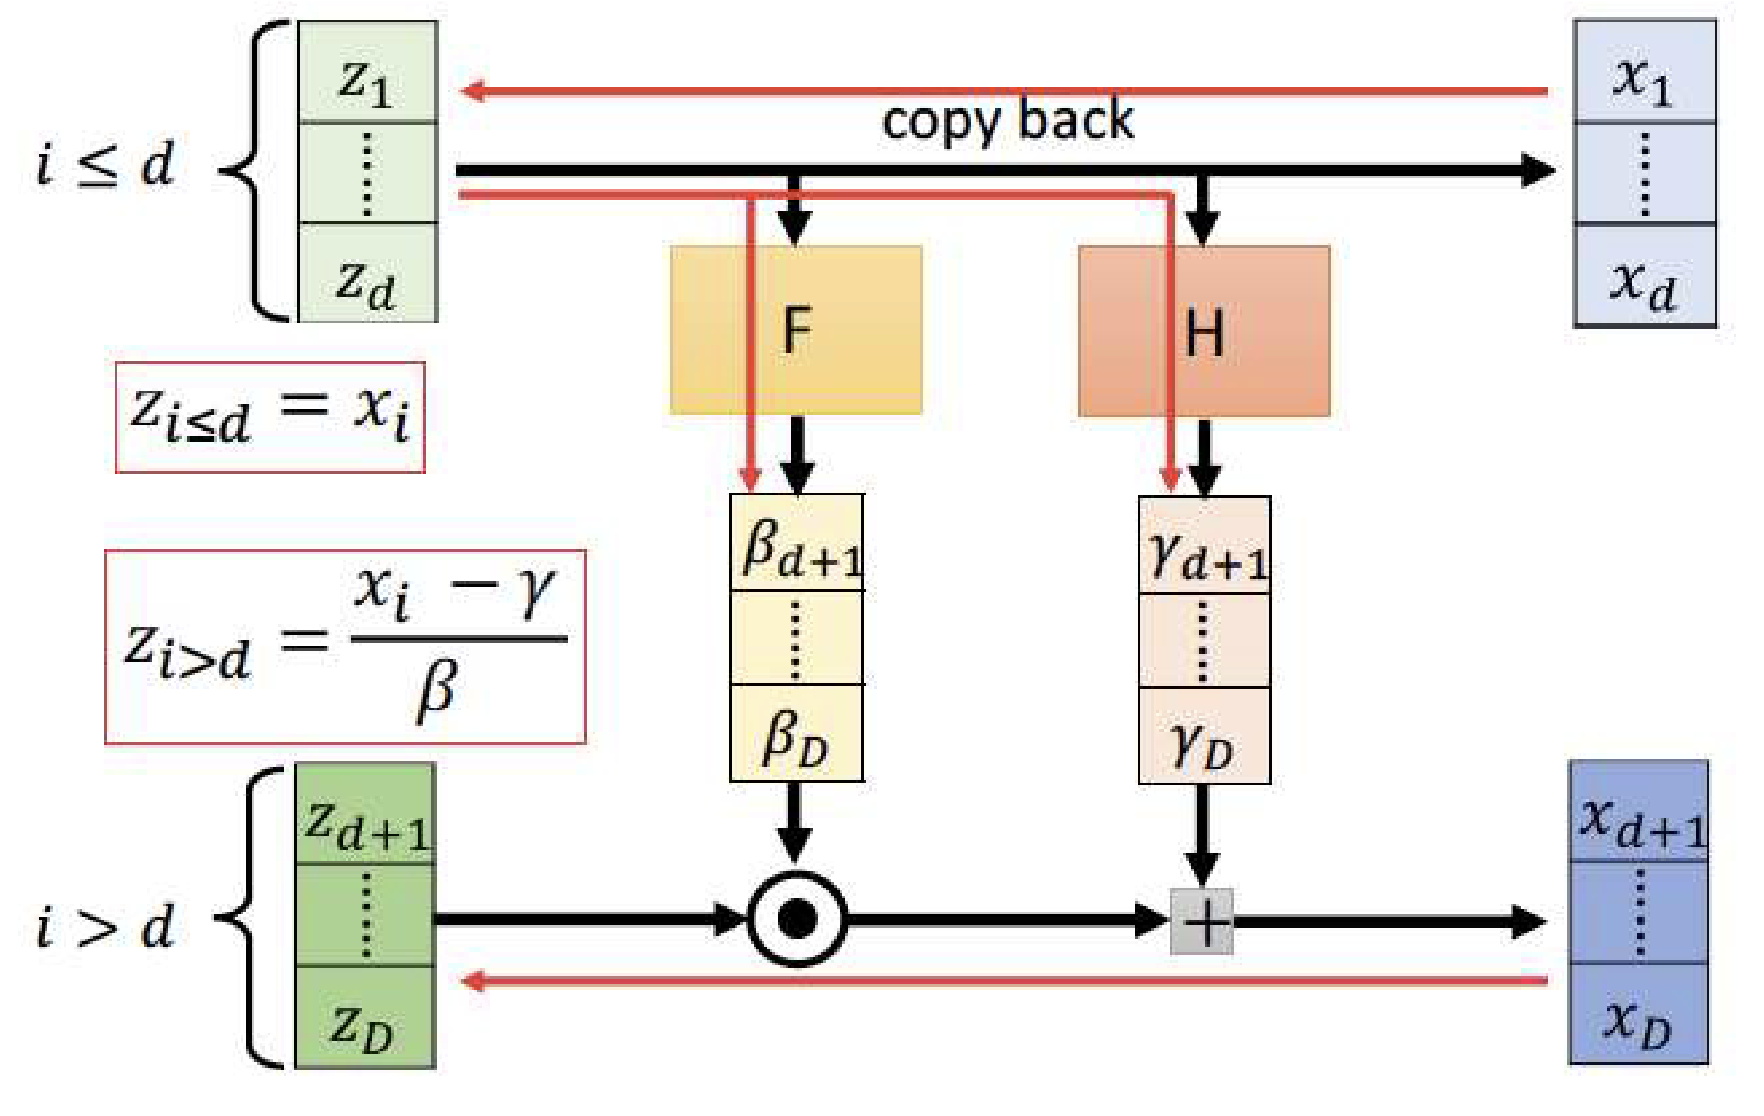
\includegraphics[width=\textwidth]{img/couple_backward.png}
        \caption{Backward pass of the coupling layer}
        \label{fig:back}
      \end{subfigure}
      \caption{Coupling layers are easily invertible. For both the forward and backward pass, we must do a forward pass through $F$ and $H$. }
      \label{fig:coupling_layer}
    \end{figure}

    Second, the determinant of this is easy to calculate since it is simply $\beta_1 \times \ldots \times \beta_{D-d}$. Therefore, we can stack these layers on top of each other, parameterized by different sequences of neural nets. 

  \subsubsection{RealNVP}

    By setting each function $f_i$ to be a cascading layer, we can model $f = f_K \circ \ldots \circ f_1$ and do the exact same normalizing flow model as mentioned before. This is pretty much NVP. 

    \begin{figure}[H]
      \centering 
      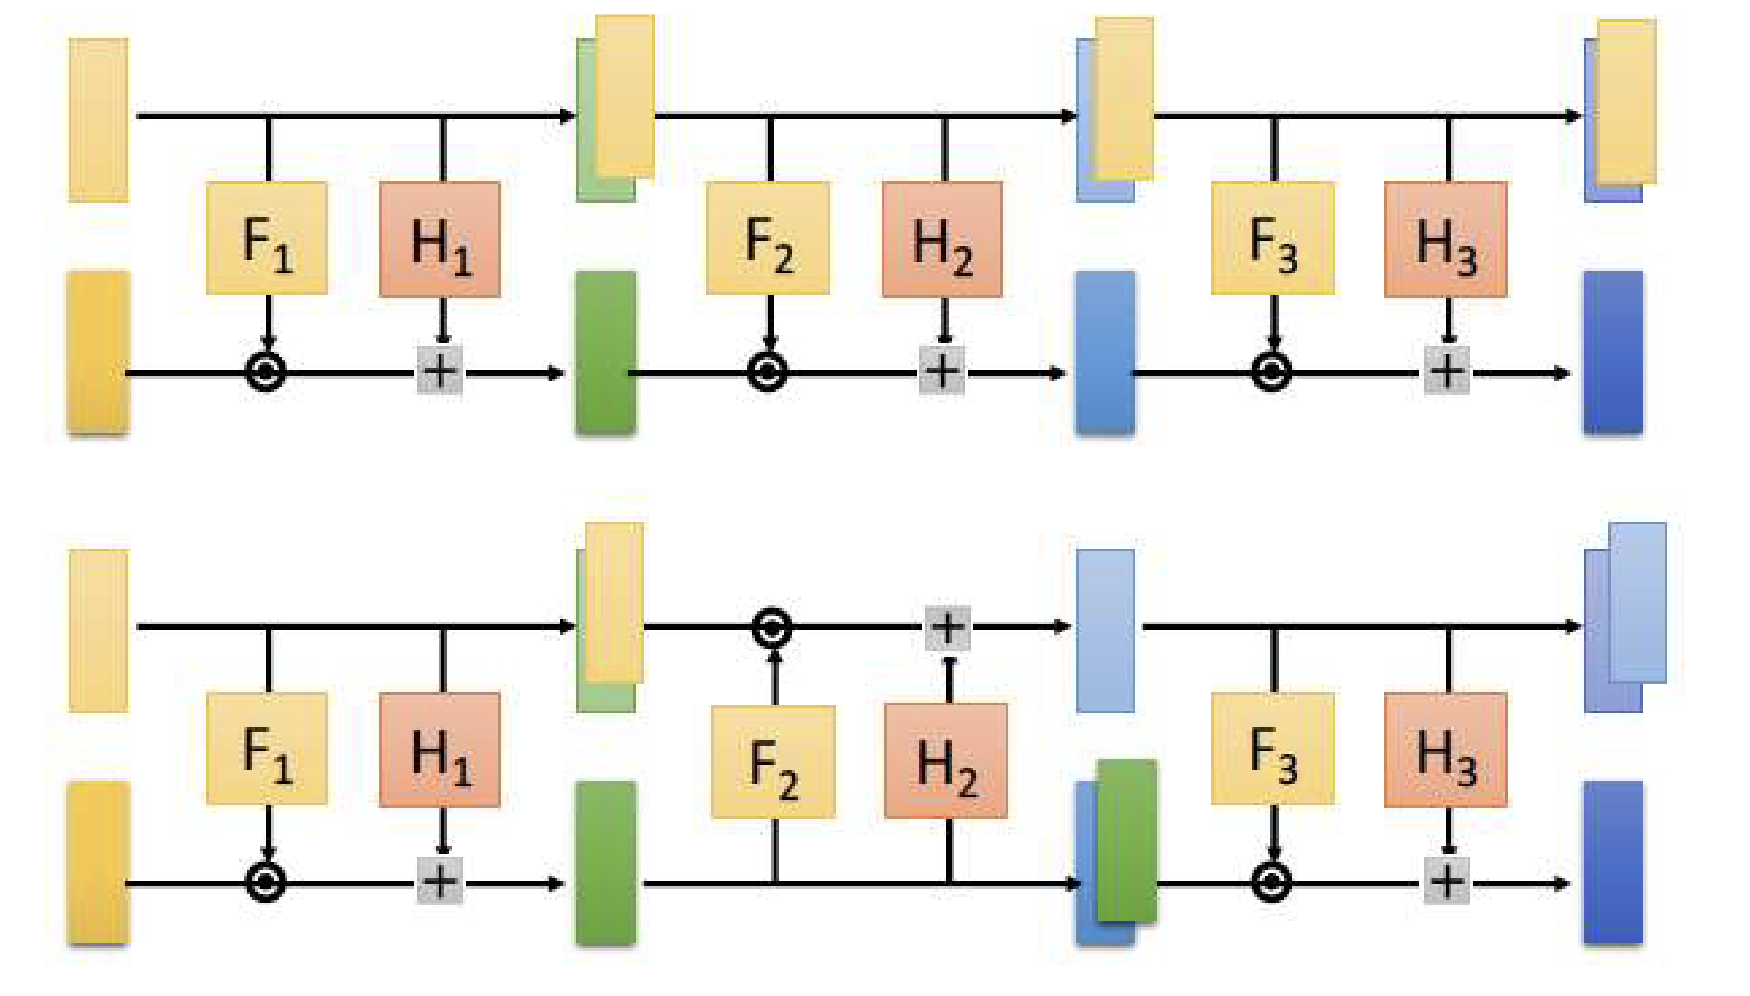
\includegraphics[scale=0.4]{img/cascading_layers.png}
      \caption{Cascading coupling layers represents $f$, where each layer is $f_i$.} 
      \label{fig:cascading_layers}
    \end{figure}

  \subsubsection{NICE}

    \textbf{Volume preserving flows} design the flow such that the Jacobian determinant is equal to $1$ (which is more restrictive but allows $O(1)$ computation) but still allows for rich posteriors. Therefore, even though computing the transformation $f_K \circ \ldots f_1$ will take longer due to the forward pass of neural nets, the lack of need to calculate the determinant keeps this fast. An example of such a volume-preserving coupling-layer flow model was introduced in \cite{nice} by Dinh in 2014. 

    \begin{definition}[NICE]
      The \textbf{nonlinear independent components estimation (NICE)} model uses \textbf{additive coupling layers} of the form 
      \begin{align}
        x_{1:d} & = z_{1:d} \\
        x_{d+1:n} & = z_{d+1:n} + H(x_{1:d})
      \end{align}
      which we can see has a Jacobian determinant of one. The final layer of NICE is a multiplication by a diagonal matrix with all diagonal elements nonzeros, i.e. $x_i = \beta_i z_i$, which is invertible and has the absolute value of the determinant $\prod_i |\beta_i|$. 
    \end{definition}

    \begin{figure}[H]
      \centering 
      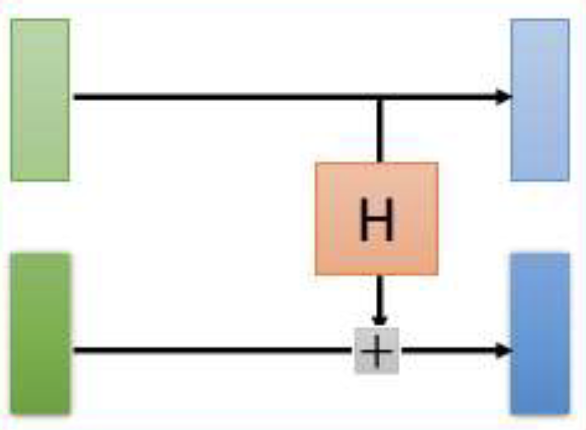
\includegraphics[scale=0.4]{img/nice_coupling.png}
      \caption{An additive coupling layer. } 
      \label{fig:nice_coupling}
    \end{figure}

\subsection{GLOW} 

  Even with all these improvements with coupling-layers, flow models did not do as well as GANs. Therefore in 2018 Kingma, having invented the VAE, made a comeback by taking flow models and adding a lot of hacks in \cite{glow} to improve it, resulting in the GLOW model. There wans't really much theoretical backing to it, but it improved normalizing flow dramatically, finally resulting in a competitor for GANs. 

  \begin{definition}[Flow Step in GLOW]
    The GLOW layer consists of 3 components. 
    \begin{enumerate}
      \item \textit{Actnorm}. 
      \item \textit{Invertible $1 \times 1$ Convolution}. 
      \item \textit{Affine Coupling Layer}. 
    \end{enumerate}
  \end{definition} 

  \begin{figure}[H]
    \centering 
    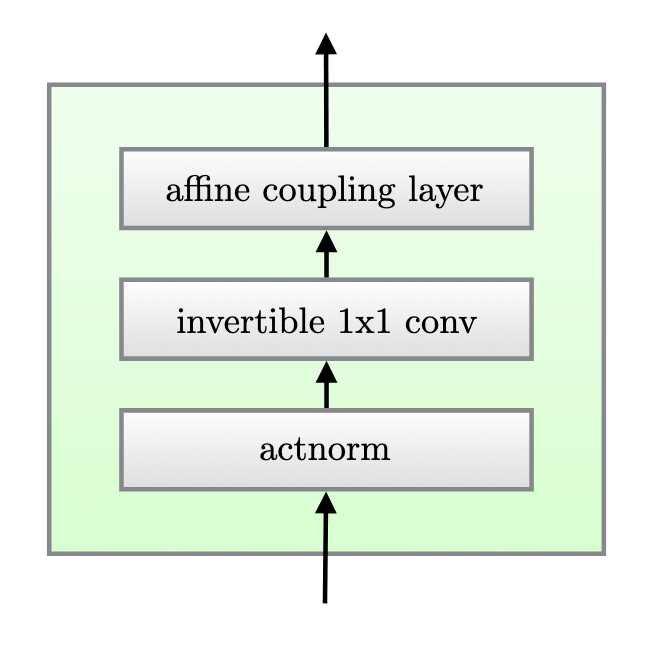
\includegraphics[scale=0.4]{img/glow_step.png}
    \caption{One step of GLOW.} 
    \label{fig:glow_step}
  \end{figure}

  After each layer, this is followed by a \textit{squeeze} operation. 

  \begin{definition}[Squeeze Operation]
    For each channel, \textbf{squeezing} divides the image into sub-squares of shape $2 \times 2 \times c$, and then reshapes them into sub-squares of shape $1 \times 1 \times 4c$. 
  \end{definition}


  \begin{definition}[Split and Concatenation Operation]
    The \textbf{split operation} passes half of the input variables to further layers and shave off the other half as ``finished.'' The \textbf{concatenation operation} performs the corresponding reverse operation: concatenation into a single tensor. 
  \end{definition}

  This results in the GLOW architecture. 

  \begin{figure}[H]
    \centering 
    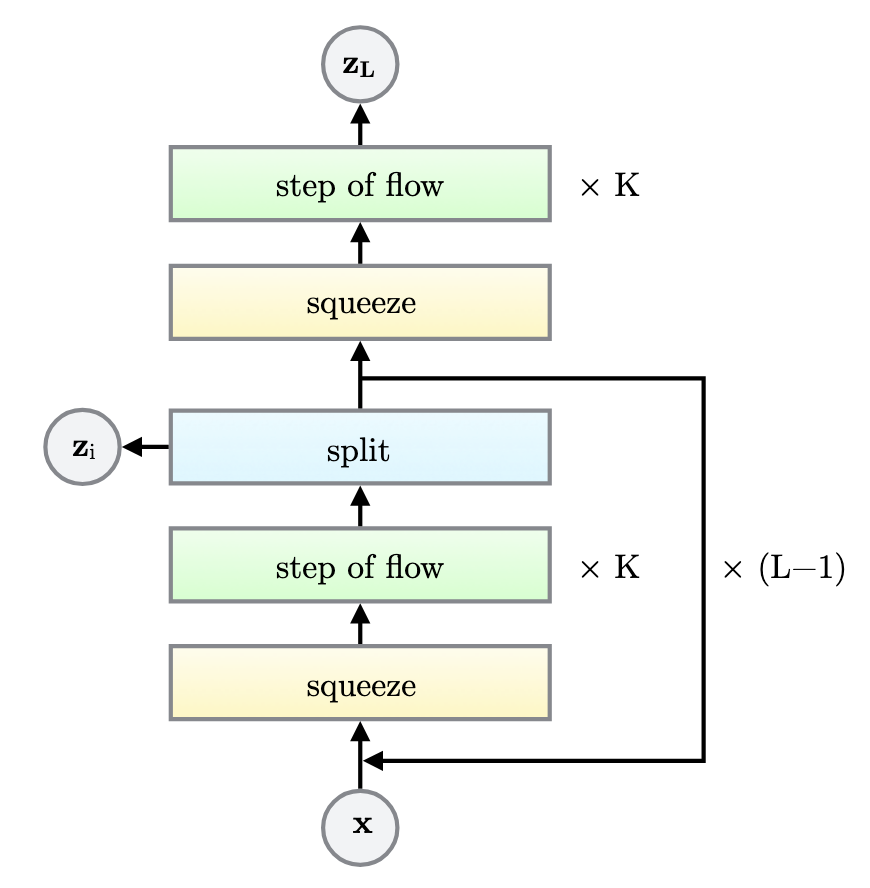
\includegraphics[scale=0.4]{img/glow_architecture.png}
    \caption{The complete glow architecture. $L = 6$ was known the be the best, but there's lots of fine-tuning. } 
    \label{fig:glow_architecture}
  \end{figure}

  You have a flow and squeeze a bunch of times is GLOW. 

  \subsubsection{c-GLOW} 
  
    There were further improvements by Lu in 2019, where in introduced conditional GLOW in \cite{cglow}. It conditions on input noise, calculates the pdf of the noise, and subtracts it. 

    There are also applications in inpainting. You condition on the visible part and sample from conditional distribution. 


\subsection{Autoregressive Flows} 

  The nice form of flow models allows us to apply this to sequential data, i.e. in autoregressive models. Given words $x_1, \ldots, x_n$, sampled from $p(x_1, \ldots, x_n) = p(x_1) \, p(x_2 \mid x_1) \ldots p(x_n \mid x_1 \ldots x_{n-1})$, we would like to generate the next word. Doing so with RNNs can require lots of computation, so we can use \textit{autoregressive models as flow models}. Consider a Gaussian nonlinear autoregressive model. 

  \begin{equation}
    p(x) = \prod_{i=1}^n p(x_i \mid x_{<i}), \text{ where } p(x_i \mid x_{<i}) = \mathcal{N} \big( \mu(x_1, \ldots, x_{i-1}), \exp(\alpha_i (x_1, \ldots, x_{i-1}))^2 \big) 
  \end{equation}
  where $\mu_i, \alpha_i$ are deep neural networks (but not too deep due to computation, e.g. they can be fixed-length input resnets). Assuming that this is optimized somehow, we can sample from a Gaussian and run it through the neural nets to get the parameters of the next Gaussian distribution, sample them, and then do it again. 
  \begin{equation}
    z_i \sim \mathcal{N}(0, 1), \qquad x_i = \mu_i + \exp(\alpha_i) z_i = \mu_i (x_{<i}) + \exp(\alpha_i (x_{<i})) z_i 
  \end{equation}

  This is the key idea to autoregressive normalizing flows. What we have just talked about is called a \textbf{masked autoregressive flow}. 

  \begin{figure}[H]
    \centering
    \begin{subfigure}[b]{0.45\textwidth}
      \centering
      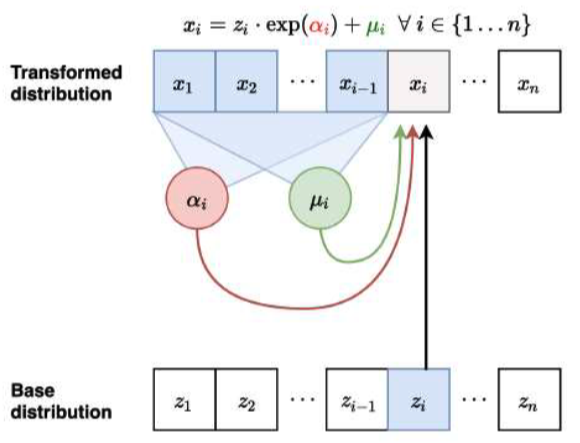
\includegraphics[scale=0.36]{img/maf.png}
      \caption{}
      \label{fig:maf}
    \end{subfigure}
    \hfill 
    \begin{subfigure}[b]{0.48\textwidth}
      \centering
      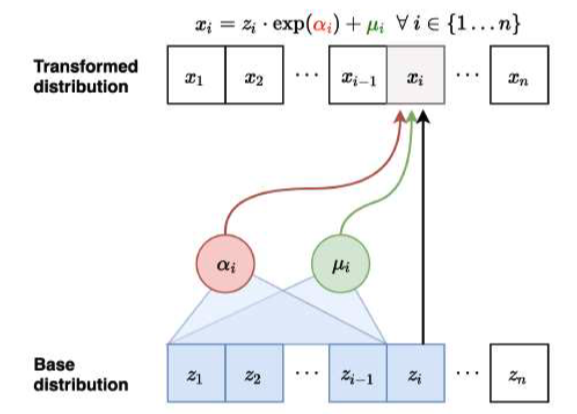
\includegraphics[width=\textwidth]{img/iaf.png}
      \caption{}
      \label{fig:iaf}
    \end{subfigure}
    \caption{}
    \label{fig:maf_vs_iaf}
  \end{figure}

  In an \textbf{inverse autoregressive flow}, the equations remain the same but the role of forward and backward passes have been reversed. 

  We can see a trade-off. 
  \begin{enumerate}
    \item \textit{Calculating log-likelihood}. MAFs are better since we can calculate it easy (remember we need determinant). IAFs requires us to go back and forth. 
    \item \textit{Sampling}. IAFs are easier since we can sample from $z_i$'s and sequentially calculate $x_i$'s. 
  \end{enumerate}

  Can we get the benefits of both? Yes, and the general idea is to train the MAF first and then have the IAF student model imitate it. 

  \begin{example}[Video Flows]
    We can model a video as as a time series generated by a fancy random Gaussian walk, where the normal distributions are transformed by a neural network. This leads to \textit{WaveNet}. 
  \end{example}

\subsection{Infinitesimal Flows} 

\subsection{Wasserstein Flows} 


\bibliographystyle{alpha}
\bibliography{./bibfile}
\end{document}

